\chapter{Εισαγωγή}
\label{ch:into}

\section{Μετοχές}
Στην σημερινή εποχή, η οποία χαρακτηρίζεται από την ευκολία στην πρόσβαση της πληροφορίας καθώς και απο την χρήση των κινητών τηλεφώνων και εφαρμογών,
η πρόσβαστη σε όλα τα χρηματηστήρια του πλανήτη δέν ήταν ποτέ πιο έυκολη.

Υπάρχει πληθώρα διαθέσιμων εφαρμογών, οι οποίες προσφέρουν την δυνατότητα στους χρήστες να επενδύσουν σε μετοχές, ομόλογα και οποιοδήποτε άλλου είδους επένδυτικού σχήματος.
Οι μετοχές είναι το πιο διαδεδομένο και γνωστό χρηματοοικονομικό προϊόν.

\subsection{Ορισμός Μετοχής}

Τι ειναι όμως οι μετοχές? Σύμφωνα με τον ορισμό του \textbf{Wikipedia}:

\begin{tcolorbox}[colframe=blue!50!black, colback=blue!5, title=Ορισμός Ομολόγου]
    \href{https://el.wikipedia.org/wiki/%CE%9C%CE%B5%CF%84%CE%BF%CF%87%CE%AE_(%CF%87%CF%81%CE%B7%CE%BC%CE%B1%CF%84%CE%BF%CE%BF%CE%B9%CE%BA%CE%BF%CE%BD%CE%BF%CE%BC%CE%B9%CE%BA%CE%AC)#:~:text=%CE%9C%CE%B5%CF%84%CE%BF%CF%87%CE%AE%20%CE%B5%CE%AF%CE%BD%CE%B1%CE%B9%20%CE%AD%CE%BD%CE%B1%20%CE%B1%CF%80%CF%8C%20%CF%84%CE%B1,%CF%83%CF%85%CE%BC%CE%BC%CE%B5%CF%84%CE%BF%CF%87%CE%AE%20%CF%84%CE%BF%CF%85%20%CF%83%CF%84%CE%B7%CE%BD%20%CE%B1%CE%BD%CF%8E%CE%BD%CF%85%CE%BC%CE%B7%20%CE%B5%CF%84%CE%B1%CE%B9%CF%81%CE%B5%CE%AF%CE%B1.}{\textbf{Μετοχή}} 
    είναι ένα από τα ίσα μερίδια, στα οποία διαιρείται το κεφάλαιο μιας ανώνυμης εταιρείας. Αυτός που κατέχει μετοχές ονομάζεται μέτοχος μίας εταιρείας. 
    Η μετοχή, ως αξιόγραφο, ενσωματώνει τα δικαιώματα του μετόχου που πηγάζουν από τη συμμετοχή του στην ανώνυμη εταιρεία. 
    Τα δικαιώματα αυτά, είναι ανάλογα του αριθμού μετοχών που κατέχει ο μέτοχος.
\end{tcolorbox}

Οι μετοχές μπορεί να διακρίνονται: 
\begin{itemize}
    \item Κοινές
    \item Προνομιούχες
    \item Επικαρπίας
    \item Ονομαστικές
    \item Ανώνυμες
    \item Με ψήφο
    \item Χωρίς ψήφο
    \item Διαπραγματεύσιμες σε Χρηματιστήριο
    \item Μη διαπραγματεύσιμες
\end{itemize}

Η \textbf{κοινή μετοχή} είναι ο πιο συνηθισμένος τύπος μετοχής και περιλαμβάνει όλα τα βασικά δικαιώματα ενός μετόχου, όπως δικαίωμα συμμετοχής στα κέρδη,
στην έκδοση νέων μετοχών, στο προϊόν της εκκαθάρισης, καθώς και δικαίωμα ψήφου στη Γενική Συνέλευση της εταιρείας και συμμετοχής στη διαχείρισή της.

Η \textbf{προνομιούχος μετοχή} προσφέρει απλά ένα προβάδισμα έναντι των κατόχων κοινών μετοχών, στη λήψη μερίσματος και στη λήψη του προϊόντος της εκκαθάρισης
σε περίπτωση διάλυσης της επιχείρησης, αλλά συνήθως στερείται του δικαιώματος ψήφου και συμμετοχής στη διαχείριση της επιχείρησης.

Σύμφωνα με τον ορισμό του \textbf{Investopedia}:

Μια μετοχή, γνωστή και ως μετοχικό κεφάλαιο, είναι ένας τίτλος που αντιπροσωπεύει την ιδιοκτησία ενός κλάσματος της εταιρείας που την εκδίδει.
Οι μονάδες μετοχών ονομάζονται μερίσματα, οι οποίες δίνουν δικαίωμα στον ιδιοκτήτη σε ένα ποσοστό των περιουσιακών στοιχείων 
και των κερδών της εταιρείας ίσο με το ποσό των μετοχών που κατέχει.

Οι μετοχές αγοράζονται και πωλούνται κυρίως σε χρηματιστήρια και αποτελούν τη βάση πολλών χαρτοφυλακίων μεμονωμένων επενδυτών.
Οι εταιρείες εκδίδουν μετοχές για να συγκεντρώσουν κεφάλαια για να λειτουργήσουν τις επιχειρήσεις τους.

\subsection{Διαφορές μετοχών και ομολόγων}

Σε αυτό το σημείο είναι σημαντικό να διαχωρίσουμε τις βασικές διαφορές μεταξύ μετοχών και ομολόγων.
Τα ομόλογα αντιπρωσοπεύουν μια άτυπη μορφή δάνειου ενώ απο την άλλη οι μετοχές αντιπροσωπεύουν μερίδιο ιδιοκτησίας σε μια εταιρεία.

\begin{itemize}
    \item \textbf{Δικαιώματα:} Στα ομόλογα ο επενδυτής δικαιούται τόκους σε τακτά χρονικά διαστήματα και την επιστροφή του αρχικού κεφαλαίου κατά τη λήξη του ομολόγου.
    Στις μετοχές ο επενδυτής μπορεί να λαμβάνει μερίσματα (εφόσον διανεμηθούν) και έχει δικαίωμα ψήφου στις γενικές συνελεύσεις της εταιρείας.
    \item \textbf{Ιδιοκτησία:} Οι κάτοχοι μετοχών είναι συνιδιοκτήτες της εταιρείας. Αντίθετα, οι κάτοχοι ομολόγων είναι πιστωτές της εταιρείας.
    \item \textbf{Προτεραιότητα σε περίπτωση πτώχευσης:} Οι ομολογιούχοι έχουν νομική προτεραιότητα σε περίπτωση πτώχευσης και αποζημιώνονται πρώτοι από την εκποίηση 
    των περιουσιακών στοιχείων. Οι μέτοχοι συνήθως δεν λαμβάνουν τίποτα.
    \item \textbf{Κίνδυνος:} Οι μετοχές είναι γενικά πιο ριψοκίνδυνες σε σύγκριση με τα ομόλογα, καθώς οι αποδόσεις τους εξαρτώνται άμεσα 
    από την κερδοφορία της εταιρείας και τις συνθήκες της αγοράς.
    \item \textbf{Απόδοση:} Τα ομόλογα παρέχουν σταθερή και προκαθορισμένη απόδοση μέσω των τόκων. Οι μετοχές μπορεί να προσφέρουν υψηλότερη απόδοση, αλλά ταυτόχρονα με μεγαλύτερη αβεβαιότητα.
    \item \textbf{Αγορά:} Οι μετοχές διαπραγματεύονται κυρίως στο χρηματιστήριο. Τα ομόλογα μπορεί να διαπραγματεύονται είτε στο χρηματιστήριο είτε εξω απο αυτό.
\end{itemize}

\subsection{Προαιρεση Μετοχών}

Μια άλλη μορφή επενδυτικής ενέργειας εκτός απο την αυτοτελή αγορά μετοχών είναι η προαιρεση μετοχών.
Σύμφωνα με τον ορισμό του \textbf{Investopedia}:
\begin{tcolorbox}[colframe=blue!50!black, colback=blue!5, title=Ορισμός Προαιρεσης Μετοχών]
    Ένα δικαίωμα προαίρεσης αγοράς μετοχών (γνωστό και ως δικαίωμα αγοράς μετοχών) 
    δίνει σε έναν επενδυτή το δικαίωμα —αλλά όχι την υποχρέωση να αγοράσει ή να πουλήσει 
    μια μετοχή σε συμφωνημένη τιμή και ημερομηνία. Το μέγεθος της προαίρεσης είναι συνήθως 100 μετοχές. 
    Υπάρχουν δύο τύποι επιλογών:
    \begin{itemize}
        \item \textbf{Puts:} Εκτίμηση ότι μια μετοχή θα πέσει
        \item \textbf{Calls:} Εκτίμηση ότι μια μετοχή θα ανέβει
    \end{itemize}
\end{tcolorbox}

Επειδή η προαίρεση έχει μερίδιο μετοχών (ή δείκτη μετοχών) ως υποκείμενο περιουσιακό της στοιχείο,
τα δικαιώματα προαίρεσης μετοχών είναι μια μορφή \textbf{παραγώγου μετοχικού κεφαλαίου} και 
μπορεί να ονομάζονται μετοχικά δικαιώματα.

Επίσης τα δικαιώματα προαίρεσης αγοράς μετοχών δύνονται σε ορισμένες περιπτώσεις σαν ένας τύπος
αποζημίωσης μετοχικού κεφαλαίου από εταιρείες σε ορισμένους υπαλλήλους ή στελέχη που ουσιαστικά 
ισοδυναμούν με δικαιώματα αγοράς. Αυτά διαφέρουν από τα δικαιώματα προαίρεσης μετοχών σε μετοχές που διαπραγματεύονται στην αγορά,
καθώς περιορίζονται σε μια συγκεκριμένη εταιρεία που τα εκδίδει στους δικούς της υπαλλήλους.

Οπότε συνοψίζοντας υπάρχουν δύο τύποι προαιρεσης μετοχών:
\begin{itemize}
    \item \textbf{Puts:} Οι επιλογές πώλησης παρέχουν στον κάτοχο το δικαίωμα, αλλά όχι την υποχρέωση, να πουλήσει το περιουσιακό στοιχείο σε μια καθορισμένη τιμή εντός συγκεκριμένου χρονικού πλαισίου.
    \item \textbf{Calls:} Δικαιώματα αγοράς παρέχουν στον κάτοχο το δικαίωμα, αλλά όχι την υποχρέωση, να αγοράσει το περιουσιακό στοιχείο σε καθορισμένη τιμή εντός συγκεκριμένου χρονικού πλαισίου.
\end{itemize}

\begin{tcolorbox}[colframe=gray!50!black, colback=gray!5, title=ΠαράδειγμαΠροαιρεσης Μετοχών]
    Εστω οτι η μετοχή Α διαπραγματεύεται στα 100 ευρώ, ένα δικαίωμα αγοράς \textbf{call} με τιμή εξάσκησης τα 120€ θα έχει νόημα να ασκηθεί δηλαδή να μετατραπεί σε μετοχές στην τιμή εξάσκησης
    μόνο εάν η τιμή της μετοχής ξεπεράσει τα 120€.

    Αντίστοιχα, ένα δικαίωμα πώλησης \textbf{put} με τιμή εξάσκησης τα 80 δολάρια θα έχει αξία μόνο εάν η τιμή της μετοχής πέσει κάτω από τα 80 δολάρια.
    Σε εκείνο το σημείο, και τα δύο δικαιώματα θα θεωρούνται \textbf{"εντός χρημάτων in the money ITM"}, που σημαίνει ότι έχουν εσωτερική αξία δηλαδή, τη διαφορά μεταξύ της τιμής εξάσκησης και της τρέχουσας τιμής της μετοχής.
    Διαφορετικά, τα δικαιώματα είναι \textbf{"εκτός χρημάτων out of the money OTM"} και αποτελούνται μόνο από εξωτερική αξία γνωστή και ως χρονική αξία.
    
    Τα δικαιώματα OTM εξακολουθούν να έχουν κάποια αξία, καθώς υπάρχει πιθανότητα η τιμή του υποκείμενου περιουσιακού στοιχείου να κινηθεί εντός χρημάτων πριν από την ημερομηνία λήξης του δικαιώματος. 
    Αυτή \textbf{η πιθανότητα αντικατοπτρίζεται στην τιμή του δικαιώματος}.
\end{tcolorbox}

Τα options (προαιρέσεις μετοχών) προσφέρουν σημαντικά πλεονεκτήματα στους επενδυτές, κυρίως λόγω της ευελιξίας και της μόχλευσης που παρέχουν.
Μέσω των options, κάποιος μπορεί:	
\begin{itemize}
    \item Να λάβει μια θετική (long) ή αρνητική (short) θέση σε μια μετοχή χωρίς να χρειάζεται να την αγοράσει ή να τη δανειστεί για πώληση.
    \item Μπορεί να επωφεληθεί από τις κινήσεις της τιμής της μετοχής, χρησιμοποιώντας σημαντικά μικρότερο κεφάλαιο σε σύγκριση με μια αντίστοιχη θέση με αγορά ή πώληση μετοχών
    \item Η δυνητική απόδοση είναι μεγαλύτερη, ενώ το ρίσκο περιορίζεται στο αρχικό ποσό που καταβλήθηκε για την αγορά του option.
\end{itemize}

Στο παρακάτω σχήμα (Σχήμα~\ref{fig:call_option})  φαίνεται ξεκάθαρα η διαφορά μεταξύ της αγοράς μετοχών και της αγοράς προαιρεσης μετοχών.
Ενώ η αγορά 100 μετοχών κοστους 50€ θα κόστιζε 5000 ευρώ, η αγορά 1 call option με τιμή εξάσκησης 53 ευρώ θα κόστιζε μόνο 300 ευρώ.
Επιπλέον, ότι η τιμή ισοσκέλισης (breakeven) για την αγορά της μετοχής είναι τα 50 δολάρια ανά μετοχή, αλλά για τη συναλλαγή με option 
η τιμή ισοσκέλισης είναι τα 53 δολάρια ανά μετοχή.
\begin{figure}[H]
    \centering
    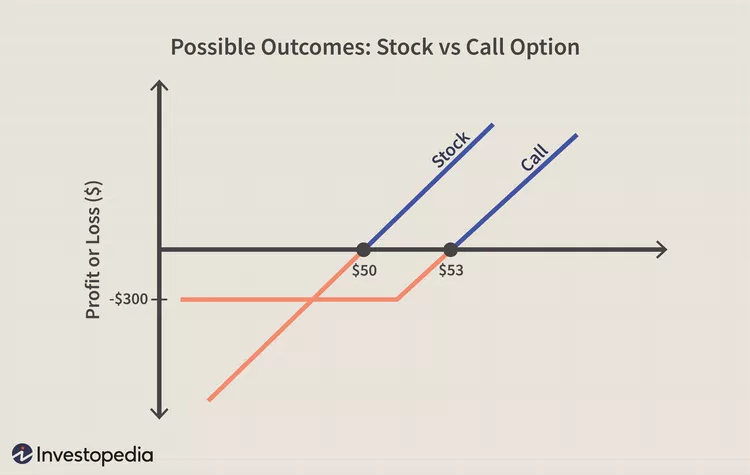
\includegraphics[width=1.0\textwidth]{figures/call_option.png}
    \caption{Παράδειγμα Call Option}
    \label{fig:call_option}
\end{figure}

To \textbf{σημαντικό} είναι οτι παρόλο που και οι δύο επενδύσεις έχουν απεριόριστο δυνητικό κέρδος, \textbf{τα πιθανά σενάρια ζημίας διαφέρουν σημαντικά}.
Χαρακτηριστικό παράδειγμα: ενώ η μέγιστη ζημία στην προαίρεση είναι τα 300 ευρώ, η ζημία από την αγορά της μετοχής μπορεί να φτάσει έως και ολόκληρη την αρχική επένδυση ,εαν η τιμή της μετοχής καταρρεύσει στο μηδέν.

\subsection{Βασικές Έννοιες}

\textbf{Ημερομηνία Λήξης (Expiration Date):}

Τα options ισχύουν μόνο για συγκεκριμένο χρονικό διάστημα, γνωστή ως \textbf{ημερομηνία λήξης}. 
Τα options με μεγαλύτερη διάρκεια μέχρι τη λήξη έχουν υψηλότερη αξία, καθώς υπάρχει μεγαλύτερη πιθανότητα η τιμή της μετοχής να κινηθεί θετικά.
Οι ημερομηνίες λήξης ορίζονται βάσει προκαθορισμένου χρονοδιαγράμματος και κυμαίνονται από
\begin{itemize}
    \item ημερήσιες
    \item εβδομαδιαίες
    \item μηνιαίες
    \item εως και ετήσιες
\end{itemize}

\textbf{Τιμή Εξάσκησης (Strike Price):}
Η \textbf{τιμή εξάσκησης} καθορίζει την τιμή που θα αποδώσει ενα option οταν/εαν ασκηθεί. Ουσιαστικά είναι η τιμή την οποία ο επενδυτής εκτιμάει ότι θα βρίσκεται η μετοχή (πάνω ή κάτω) μέχρι την ημερομηνία λήξης.

\textbf{Επιτόπια Τιμή (Spot Price):}
Η \textbf{spot price} είναι η τρέχουσα τιμή της μετοχής στην αγορά. Είναι η τιμή που θα πληρώνε ο επενδυτής για να αγοράσει τη μετοχή σήμερα.

\textbf{Μεταβλητότητα (Volatility):}
Η μεταβλητότητα της τιμής μιας μετοχής ορίζεται ως η τάση της τιμής να παρουσιάζει διακυμάνσεις με την πάροδο του χρόνου. Υψηλή μεταβλητότητα υποδηλώνει ότι η τιμή της μετοχής μπορεί να μεταβάλλεται γρήγορα και απρόβλεπτα, αυξάνοντας έτσι την αξία των options.

\textbf{Υπολογισμός Μεταβλητότητας (Volatility):}

Η μεταβλητότητα μπορεί να υπολογιστεί χρησιμοποιώντας τον παρακάτω τύπο:

\begin{equation}
    \sigma = \sqrt{\frac{1}{N-1} \sum_{i=1}^{N} (r_i - \bar{r})^2}
\end{equation}

όπου:
\begin{itemize}
    \item $\sigma$: Η τυπική απόκλιση (μεταβλητότητα)
    \item $N$: Ο αριθμός των παρατηρήσεων
    \item $r_i$: Η απόδοση της μετοχής για την $i$-οστή περίοδο
    \item $\bar{r}$: Η μέση απόδοση της μετοχής
\end{itemize}

Οπου η μέση τιμή ($\bar{r}$) υπολογίζεται απλοικά με τον παρακάτω τύπο:
\begin{equation}
    \bar{r} = \frac{1}{N} \sum_{i=1}^{N} r_i
\end{equation}

\textbf{Eπιτόκιο ανευ κινδύνου (Risk Free Rate):}
Το επιτόκιο χωρίς κίνδυνο (risk-free rate) αντιπροσωπεύει το επιτόκιο που θα περίμενε ένας επενδυτής από μια απολύτως ασφαλή επένδυση για μια συγκεκριμένη χρονική περίοδο.
Ο λεγόμενος "πραγματικός" ρυθμός χωρίς κίνδυνο μπορεί να υπολογιστεί αφαιρώντας τον τρέχοντα ρυθμό πληθωρισμού από την απόδοση ενός κρατικού ομολόγου που αντιστοιχεί στη διάρκεια της επένδυσης.
Η τιμή αυτή κυμαίνεται ως συνήθως μεταξύ 2.5\% και 5.5\% ετησίως.

\subsection{Ιστορική Αναδρομή}
Το \textbf{μοντέλο Black-Scholes} είναι μία από τις σημαντικότερες έννοιες της σύγχρονης χρηματοοικονομικής θεωρίας.
Γνωστό και ως μοντέλο Black-Scholes-Merton (BSM), αυτή η μαθηματική εξίσωση εκτιμά τη θεωρητική αξία ενός option, λαμβάνοντας υπόψη την επίδραση του χρόνου και άλλων παραγόντων κινδύνου.
Το μοντέλο Black-Scholes, το οποίο αναπτύχθηκε το 1973 από τους Fischer Black, Robert Merton και Myron Scholes, 
ήταν η πρώτη ευρέως χρησιμοποιούμενη μαθηματική μέθοδος για τον υπολογισμό της θεωρητικής αξίας ενός συμβολαίου δικαιωμάτων προαίρεσης.
Χρησιμοποιεί τις τρέχουσες τιμές των μετοχών, τα αναμενόμενα μερίσματα, την τιμή άσκησης του δικαιώματος προαίρεσης, τα αναμενόμενα επιτόκια, το χρόνο μέχρι τη λήξη και την αναμενόμενη μεταβλητότητα.

Η αρχική εξίσωση εισήχθη στην εργασία των Black και Scholes το 1973, \textbf{«The Pricing of Options and Corporate Liabilities»}, που δημοσιεύθηκε στο Journal of Political Economy.
Ο Robert C. Merton ο οποίος βοήθησε στην επιμέλεια του άρθρου, δημοσίευσε το δικό του άρθρο στο The Bell Journal of Economics and Management Science αργότερα την ίδια χρονιά:
\textbf{«Theory of Rational Option Pricing» (Θεωρία της ορθολογικής τιμολόγησης δικαιωμάτων προαίρεσης)}.
διεύρυνοντας τη μαθηματική κατανόηση και τις εφαρμογές του μοντέλου.

Για αυτό το έργο οι Scholes και Merton τιμήθηκαν με το βραβείο \textbf{Νόμπελ Οικονομικών Επιστημών το 1997}.

\subsection{Αλγόριθμος Black Scholes}

H εξίσωση του μοντέλου θεωρεί ότι μέσα όπως μετοχές ή συμβόλαια μελλοντικής εκπλήρωση:
\begin{itemize}
    \item θα έχουν μια λογαριθμοκανονική κατανομή των τιμών
    \item θα ακολουθεί έναν τυχαίο περίπατο με σταθερή μετατόπιση και μεταβλητότητα.
\end{itemize}

Η εξίσωση χρησιμοποιεί αυτή την υπόθεση και συνυπολογίζει άλλες σημαντικές μεταβλητές για να προκύψει η τιμή ενός δικαιώματος αγοράς ευρωπαϊκού τύπου.

Το μοντέλο Black-Scholes απαιτεί τις πέντε μεταβλητές που αναλύθηκαν προηγουμένως:
\begin{itemize}
    \item την τιμή άσκησης ενός δικαιώματος προαίρεσης
    \item την τρέχουσα τιμή της μετοχής
    \item το χρόνο μέχρι τη λήξη
    \item το επιτόκιο χωρίς κίνδυνο
    \item και τη μεταβλητότητα.
\end{itemize}

Επίσης περεταίρω παραδοχές που πρέπει να αναφερθούν είναι:

\begin{itemize}
    \item Κατά τη διάρκεια της διάρκειας του δικαιώματος προαίρεσης δεν καταβάλλονται μερίσματα.
    \item Οι αγορές είναι τυχαίες επειδή οι κινήσεις της αγοράς δεν μπορούν να προβλεφθούν.
    \item Δεν υπάρχουν έξοδα συναλλαγής κατά την αγορά του δικαιώματος προαίρεσης.
    \item Το επιτόκιο χωρίς κίνδυνο και η μεταβλητότητα του υποκείμενου περιουσιακού στοιχείου είναι γνωστά και σταθερά.
    \item Οι αποδόσεις του υποκείμενου περιουσιακού στοιχείου κατανέμονται κανονικά.
    \item Το δικαίωμα προαίρεσης είναι ευρωπαϊκό και μπορεί να ασκηθεί μόνο κατά τη λήξη.
\end{itemize}

Ο τύπος του Black-Scholes υπολογίζεται πολλαπλασιάζοντας την τιμή της μετοχής με τη συνάρτηση τυπικής κατανομής πιθανοτήτων.
Η καθαρή παρούσα αξία (ΚΠΑ) της τιμής εξάσκησης πολλαπλασιαζόμενη με τη συσωρευτική τυπική κανονική κατανομή και αφαιρείται στη συνέχεια από την προκύπτουσα τιμή του προηγούμενου υπολογισμού.

\begin{equation}
    C = S_0 N(d_1) - X e^{-rT} N(d_2)
\end{equation}

όπου:
\begin{itemize}
    \item $C$: Η τιμή του δικαιώματος προαίρεσης
    \item $S_0$: Η τρέχουσα τιμή της μετοχής
    \item $X$: Η τιμή άσκησης του δικαιώματος προαίρεσης
    \item $r$: Το επιτόκιο χωρίς κίνδυνο
    \item $T$: Ο χρόνος μέχρι τη λήξη
    \item $N(d)$: Η συνάρτηση κατανομής κανονικής πιθανότητας
\end{itemize}

Τα $d_1$ και $d_2$ υπολογίζονται με τους παρακάτω τύπους:
\begin{equation}
    d_1 = \frac{\ln(\frac{S_0}{X}) + (r + \frac{\sigma^2}{2})T}{\sigma \sqrt{T}}
\end{equation}
\begin{equation}
    d_2 = d_1 - \sigma \sqrt{T}
\end{equation}

και το N(d) είναι η συνάρτηση κατανομής κανονικής πιθανότητας, που υπολογίζεται με τον παρακάτω τύπο:
\begin{equation}
    N(d) = \frac{1}{\sqrt{2\pi}} \int_{-\infty}^{d} e^{-\frac{x^2}{2}} dx
\end{equation}

\subsection{Σημασία της Θεωρίας}
Το μοντέλο Black-Scholes κατέχει μεγάλη σημασία στον οικονομικό χώρο διότι εισήγαγε μια αυστηρή μαθηματική προσέγγιση για την τιμολόγηση των δικαιωμάτων προαίρεσης,
επιτρέποντας στους επενδυτές και στους διαχειριστές κινδύνου να εκτιμήσουν με ακρίβεια την αξία αυτών των χρηματοοικονομικών εργαλείων.
Πριν από την ανάπτυξή του, η τιμολόγηση των options βασιζόταν κυρίως σε εμπειρικές μεθόδους ή σε υποκειμενικές εκτιμήσεις.

Η επαναστατικότητα του μοντέλου έγκειται στα εξής:
\begin{itemize}
    \item \textbf{Αυστηρή Θεωρητική Βάση:} Το μοντέλο βασίζεται σε θεμελιώδεις αρχές των μαθηματικών και της στατιστικής, όπως η κανονική κατανομή και η στοχαστική ανάλυση.
    \item \textbf{Απλοποίηση της Τιμολόγησης:} Παρέχει έναν απλό και πρακτικό τύπο για την τιμολόγηση των ευρωπαϊκών δικαιωμάτων προαίρεσης, μειώνοντας την πολυπλοκότητα της διαδικασίας.
    \item \textbf{Ενίσχυση της Αγοράς Παραγώγων:} Η εφαρμογή του μοντέλου συνέβαλε στην ανάπτυξη και την ωρίμανση της αγοράς παραγώγων, καθιστώντας την πιο διαφανή και αποτελεσματική.
    \item \textbf{Διαχείριση Κινδύνου:} Το μοντέλο επιτρέπει στους επενδυτές να αντισταθμίσουν κινδύνους (hedging) με μεγαλύτερη ακρίβεια, βελτιώνοντας τη στρατηγική τους.
    \item \textbf{Επιστημονική Αναγνώριση:} Η απονομή του Βραβείου Νόμπελ στους δημιουργούς του υπογραμμίζει τη σημασία του για τη χρηματοοικονομική επιστήμη.
\end{itemize}

Η εισαγωγή του μοντέλου Black-Scholes άλλαξε ριζικά τον τρόπο με τον οποίο οι αγορές αντιλαμβάνονται και διαχειρίζονται τα δικαιώματα προαίρεσης, καθιστώντας το ένα από τα πιο σημαντικά επιτεύγματα στη χρηματοοικονομική μηχανική.

\section{Field Programmable Gate Arrays (FPGAs)}
\label{sec:fpgas}

Τα FPGAs είναι προγραμματιζόμενα ολοκληρωμένα κυκλώματα που μπορούν να προγραμματιστούν για να εκτελούν συγκεκριμένες λειτουργίες.
Ο προγραμματισμός τους γίνεται πιό κοντά στο hardware σε σχέση με τις παραδοσιακές γλώσσες προγραμματισμού, όπως η C/C++.
Αυτό τους επιτρέπει να είναι πιο αποδοτικά σε σχέση με τις παραδοσιακές CPU και GPU, καθώς μπορούν να εκτελούν πολλές λειτουργίες ταυτόχρονα αφου έχει σχεδιαστεί πρώτα
σε μια γλώσσα περιγραφής υλικού (HDL) όπως η VHDL ή Verilog.
Τα FPGAs είναι ιδανικά για εφαρμογές που απαιτούν υψηλή απόδοση και χαμηλή καθυστέρηση, όπως η επεξεργασία σήματος, η κρυπτογραφία και οι χρηματοοικονομικές εφαρμογές.
Τα FPGAs είναι επίσης ευέλικτα και μπορούν να επαναπρογραμματιστούν για να εκτελούν διαφορετικές λειτουργίες, γεγονός που τα καθιστά ιδανικά για εφαρμογές που απαιτούν προσαρμογή και ευελιξία.

\subsection{Πλεονεκτήματα FPGAs}

\begin{itemize}
    \item \textbf{Ευελιξία:} Τα FPGAs μπορούν να προγραμματιστούν για να εκτελούν διαφορετικές λειτουργίες.
    \item \textbf{Υψηλή Απόδοση:} Τα FPGAs είναι ικανά να εκτελούν πολλές λειτουργίες ταυτόχρονα.
    \item \textbf{Χαμηλή Κατανάλωση Ενέργειας:} Τα FPGAs είναι πιο αποδοτικά σε σχέση με τις παραδοσιακές CPU και GPU.
    \item \textbf{Ευκολία Ανάπτυξης:} Τα FPGAs είναι ευκολότερα στην ανάπτυξη σε σχέση με τις παραδοσιακές CPU και GPU.
    \item \textbf{Ασφάλεια:} Τα FPGAs είναι πιο ασφαλή σε σχέση με τις παραδοσιακές CPU και GPU.
    \item \textbf{Διαθεσιμότητα:} Τα FPGAs είναι διαθέσιμα σε πολλές διαφορετικές μορφές και μεγέθη.
    \item \textbf{Επικοινωνία:} Τα FPGAs είναι ικανά να επικοινωνούν με άλλες συσκευές και συστήματα.
    \item \textbf{Επεκτασιμότητα:} Τα FPGAs είναι ικανά να επεκτείνονται για να υποστηρίξουν περισσότερες λειτουργίες και εφαρμογές.
    \item \textbf{Συμβατότητα:} Τα FPGAs είναι συμβατά με πολλές διαφορετικές γλώσσες προγραμματισμού και εργαλεία ανάπτυξης.
    \item \textbf{Αξιοπιστία:} Τα FPGAs είναι αξιόπιστα και ανθεκτικά σε σχέση με τις παραδοσιακές CPU και GPU.
\end{itemize}

\section{Στόχος και Δομή Πτυχιακής Εργασίας}